\documentclass[11pt,fleqn]{article}
%\usepackage{CJK}
\usepackage{latexsym}
\usepackage{color}
\usepackage{graphicx, float}\usepackage{graphicx}
\usepackage{algorithmic}
\usepackage{algorithm}
%\usepackage{algpseudocode}
%\usepackage[colorlinks]{hyperref}
\usepackage[toc,page]{appendix}
\usepackage{bm}
\setlength{\oddsidemargin}{-0.0in}
\setlength{\evensidemargin}{-0.0in} \setlength{\textwidth}{6.0in}
\setlength{\textheight}{9.0in} \setlength{\topmargin}{-0.2in}
%\usepackage[boxruled]{algorithm2e}

%\setlength{\leftmargin}{0.7in}
\usepackage{amssymb, graphicx, amsmath}  %  fancyheadings,
\usepackage{setspace}
\newcommand\qed{\qquad $\square$}
\newcommand{\nn}{\nonumber}

\usepackage{lipsum}

\usepackage{listings}
\lstset{
  basicstyle=\ttfamily,
  columns=fullflexible,
  frameround=fttt,
  breaklines=true,
  %postbreak=\mbox{\textcolor{red}{$\hookrightarrow$}\space},
}

\definecolor{mGreen}{rgb}{0,0.6,0}
\definecolor{mGray}{rgb}{0.5,0.5,0.5}
\definecolor{mPurple}{rgb}{0.58,0,0.82}
\definecolor{backgroundColour}{rgb}{0.95,0.95,0.92}

\lstdefinestyle{CStyle}{
    backgroundcolor=\color{backgroundColour},   
    commentstyle=\color{mGreen},
    keywordstyle=\color{magenta},
    numberstyle=\tiny\color{mGray},
    stringstyle=\color{mPurple},
    basicstyle=\footnotesize,
    breakatwhitespace=false,         
    breaklines=true,                 
    captionpos=b,                    
    keepspaces=true,                 
    numbers=left,                    
    numbersep=5pt,                  
    showspaces=false,                
    showstringspaces=false,
    showtabs=false,                  
    tabsize=2,
    language=C
}

\def \[{\begin{equation}}
\def \]{\end{equation}}
\def\proof{{\bf Proof:\quad}}
\def \endzm {\quad $\Box$}
\def\dist{\hbox{dist}}

\usepackage{tabularx,booktabs}
\newcolumntype{C}{>{\centering\arraybackslash\hsize=.5\hsize}X} % centered version of "X" type
\setlength{\extrarowheight}{1pt}
\usepackage{caption}% <-- added


\newcommand{\R}{\mathbb{R}}
%\newtheorem{yinli}{����}[section]
\newcommand{\D}{\displaystyle}
\newcommand{\T}{\textstyle}
\newcommand{\SC}{\scriptstyle}
\newcommand{\FT}{\footnotesize}

\usepackage{hyperref}
\newcommand\fnurl[2]{%
  \href{#2}{#1}\footnote{\url{#2}}%
}


%\newtheorem{theorem}{Theorem}[section]
%\renewcommand{\thetheorem}{\arabic{section}.\arabic{theorem}}
\newtheorem{definition}{Definition}
\renewcommand{\thedefinition}{\arabic{section}.\arabic{definition}}
\newtheorem{lemma}{Lemma}[section]
\renewcommand{\thelemma}{\arabic{section}.\arabic{lemma}}
\newtheorem{remark}{Remark}
\renewcommand{\theremark}{\arabic{section}.\arabic{remark}}
\newtheorem{proposition}{Proposition}[section]
\renewcommand{\theproposition}{\arabic{section}.\arabic{proposition}}
\newtheorem{corollary}{Corollary }[section]
\renewcommand{\thecorollary}{\arabic{section}.\arabic{corollary}}
\renewcommand{\theequation}{\arabic{section}.\arabic{equation}}
\renewcommand{\baselinestretch}{1.35}
\newtheorem{exam}{Example}[section]
\renewcommand{\theexam}{\arabic{section}.\arabic{exam}}
\newtheorem{theo}{Theorem}[section]
\renewcommand{\thetheo}{\arabic{section}.\arabic{theo}}

% Define a \HEADER{Title} ... \ENDHEADER block
\makeatletter
\newcommand{\HEADER}[1]{\ALC@it\underline{\textsc{#1}}\begin{ALC@g}}
\newcommand{\ENDHEADER}{\end{ALC@g}}
\makeatother

\newcommand{\argmin}{\operatornamewithlimits{argmin}}
\newcommand{\argmax}{\operatornamewithlimits{argmax}}

\usepackage{url} % to make url in bibtex shows up

\begin{document}
%\begin{CJK*}{GBK}{song}

\begin{center}

{\LARGE \bf CS380L: Advanced Operating Systems Lab \#0}\\

\vskip 25pt
 {Zeyuan Hu \footnote{20 hours spent on this lab.}, iamzeyuanhu@utexas.edu }\\
\vskip 5pt
{\small EID:zh4378 Spring 2018 }

\end{center}

\begin{spacing}{1.5}
\section{Introduction}

\noindent In this writeup, we demonstrate the steps to compile and boot the Linux 
kernel on the KVM-qemu virtual machine. We time the OS bootup time using both timer
and RTC, real-time clock in Linux and explain the value difference using the 
difference between system time and RTC. We also trace the kernel during the execution
of a test program \texttt{testprog} and we explain the difference between 
\lstinline|/dev/random| and \lstinline|/dev/urandom|.

\section{Environment}

We use a machine that has 4 Intel(R) Core(TM) i5-6200U CPU @ 2.30GHz processors and 4GB of memory. The machine runs 
Ubuntu 16.04.3 (kernel version 4.4.0-116-generic).

KVM is enabled on the machine, and we use QEMU (version 2.5.0) \footnote{\lstinline|qemu-system-x86_64 --version|} to create and run a VM for the lab. 
The VM runs a Ubuntu 16.04 with the kernel we built (version 4.15.9).

\section{Getting a VM running in KVM}

We use the Ubuntu cloud image to setup the VM. The image for QEMU can be downloaded from 
\url{https://cloud-images.ubuntu.com/releases/16.04/release/ubuntu-16.04-server-cloudimg-amd64-disk1.img}. We 
use the cloud image instead of the regular desktop image to save space (e.g., We do not need to have GUI installed).

Ubuntu cloud image needs additional metadata to boot (mainly containing the login password). 
The metadata can be provided via a seed image \cite{cloud}. To create a seed image, 
we first create a file \texttt{my-user-data} with contents:

\begin{lstlisting}
#cloud-config
password: passw0rd
chpasswd: { expire: False }
ssh_pwauth: True
\end{lstlisting}

Then we create the seed image by running:

\begin{lstlisting}
sudo apt-get install cloud-utils
cloud-localds my-seed.img my-user-data
\end{lstlisting}

We then use the downloaded Ubuntu cloud image to create root disk image for the VM 
\footnote{The default virtual size is 2G, we can resize the image via \lstinline|qemu-img resize my-disk.img +10G|. We add additional
10G in this case.}:

\begin{lstlisting}
qemu-img create -f qcow2 \
-b ubuntu-16.04-server-cloudimg-amd64-disk1.img \
my-disk.img 15G
\end{lstlisting}

Now, we are ready to boot up our VM:

\begin{lstlisting}
qemu-system-x86_64 \
-enable-kvm -curses \
-m 512 -smp 4 -redir tcp:4444::22 \
-hda my-disk.img -hdb my-seed.img"
\end{lstlisting}

This will start a VM with 4 CPU cores and 512MB of memory. We redirect port 4444 of local machine to port 22 of the VM in order to login the VM via 
SSH. The VM will run in the terminal, and login with user name \texttt{ubuntu} and \texttt{passw0rd} set in \texttt{my-user-data}. The login screen
of VM is shown in Figure \ref{login}. Once we have our VM boot up, we can remote access it via SSH from host \lstinline|ssh -p 4444 ubuntu@localhost|.

\begin{figure}
\centering
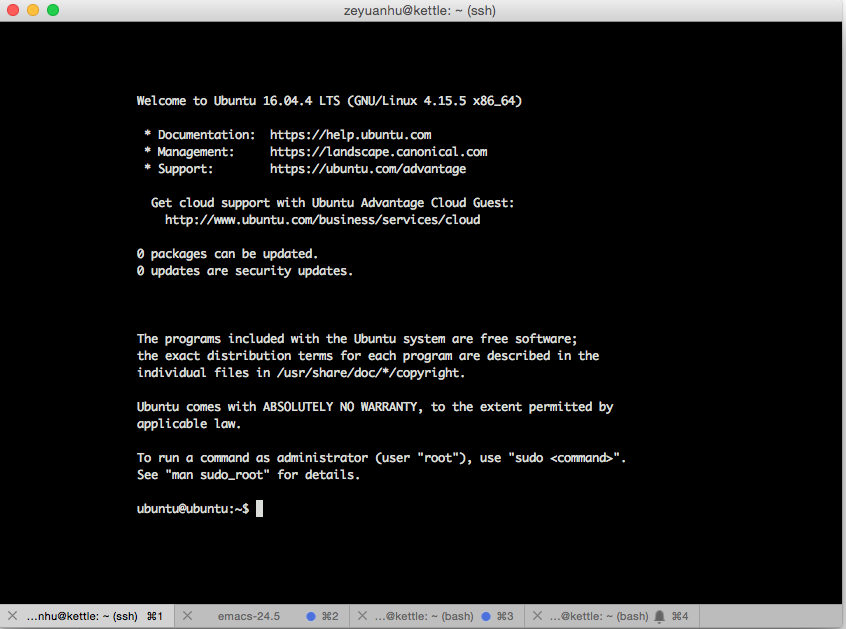
\includegraphics[scale=0.4]{bootup.png} 
\caption{Login screen of our VM}
\label{login}
\end{figure}

\section{Obtaining and building the kernel}

We first obtain the Linux Kernel source via \lstinline|wget https://cdn.kernel.org/pub/linux/kernel/v4.x/linux-4.15.9.tar.xz|.
Then, we extract the files using \lstinline|tar -xJf linux-4.15.9.tar.xz|. We make a new directory \texttt{kbuild2} as the build
directory for kernel and inside the directory, we generate \texttt{.config} file using \lstinline|make -C ../linux-4.15.9 O=$(pwd) x86_64_defconfig|.
Note that generating the \texttt{.config} file like this automatically set \texttt{CONFIG\_SATA\_AHCI=y}.
We run \lstinline|make -j16| \footnote{\texttt{-j16} means 16 threads are used, which can speed up the build process}to build the kernel.

\section{Installing and Copying Kernel Modules} 

We install the newly-built kernel by first making a new directory called \texttt{kinstall2} as a sibling of 
\texttt{kbuild2}. \texttt{kinstall2} will contain the built kernel modules. Inside \texttt{kbuild2}, we run
\lstinline|make INSTALL_MOD_PATH=../kinstall2 modules_install|.

We can see \texttt{lib} directory inside \texttt{kinstall2}, which has to be copied to the root file system of the VM. 
We notice there are two symbolic links \texttt{build} and \texttt{source} inside \texttt{kinstall2/lib/modules/4.15.9}, 
which links to the built kernel image and the source of the kernel. 
They are useless but may cause problems when copying files to the VM. Thus we just delete them. Next, we copy
the entire \text{4.15.9} directory to \texttt{/lib/modules} in the guest system by doing
\lstinline|scp -P 4444 -r 4.15.9/ ubuntu@localhost:/home/ubuntu| and inside the guest sytem, do 
\lstinline|sudo mv 4.15.9/ /lib/modules/|. Optionally, we modify \texttt{/etc/default/grub} and
delete \texttt{GRUB\_HIDDEN\_TIMEOUT\_QUIET} and increase \texttt{GRUB\_DEFAULT\_timeout} to 5 seconds. 
This modification allows us to select which kernel to boot on startup. We then run \lstinline|sudo update-grub2|.


\section{Booting KVM with your new Kernel}

We can now start VM with our own Linux kernel. The shell command we run now:

\begin{lstlisting}
qemu-system-x86_64 \
-enable-kvm -curses \
-m 512 -smp 4 -redir tcp:4444::22 \
-hda my-disk.img -hdb my-seed.img \
-kernel ~/kbuild2/arch/x86_64/boot/bzImage \
-append "root=/dev/sda1"
\end{lstlisting}

Note that we append two new options \texttt{-kernel} and \texttt{-append} to \texttt{QEMU}. 
\texttt{-kernel} option tells the location of the kernel to use, and \texttt{-append} option suggests the parameters to start the kernel. 
The \texttt{root} parameter suggests the disk partition used as root file system. 
After login, use \lstinline|uname -r| to check the kernel version string, which is shown in Figure \ref{new}.

\begin{figure}
\centering
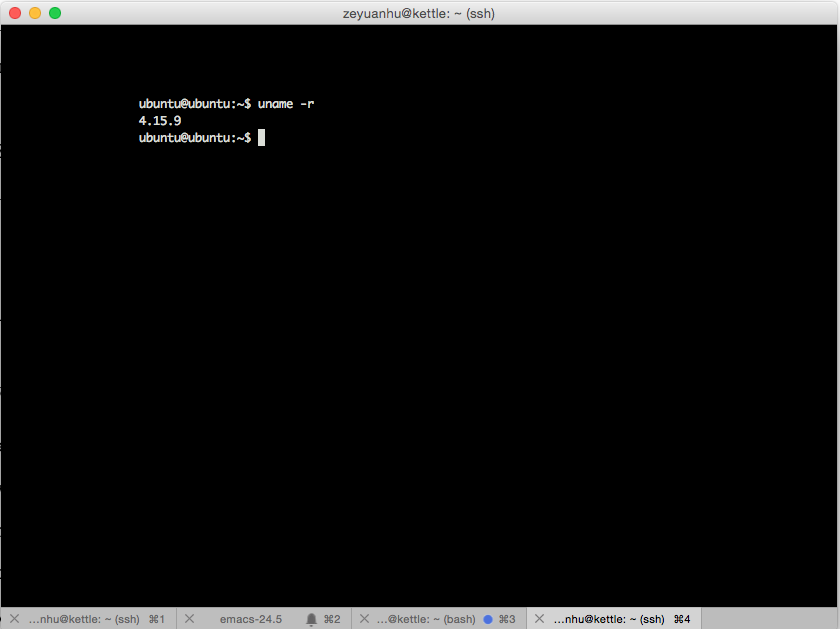
\includegraphics[scale=0.5]{new-kernel.png} 
\caption{VM with our newly-built kernel}
\label{new}
\end{figure}

\section{Booting, kernel modules, and discovering devices}

The wall clock time (tracked using a timer) for our boot takes 9.65 seconds while the time reported by the Kernel takes 7.89 seconds.
This difference may be due to the human delay on stopping the timer and also due to a disagreement between human and OS on how to define
boot finish status. Here, we stop our timer when we see the login interface but the last line of \texttt{dmesg}
\footnote{\texttt{dmesg} is used to inspect the kernel ring buffer, which contains the system log during kernel boot.} indicating this disagreement. 

\begin{lstlisting}
[    7.888123] new mount options do not match the existing superblock, will be ignored
\end{lstlisting}

To eliminate the potential human error, we use real-time clock in Linux system to time the difference between the wall clock time and the time 
reported by Kernel.

\begin{lstlisting}
$ dmesg -T | grep "RTC time"
[Tue Mar 13 12:59:33 2018] RTC time: 12:59:34, date: 03/13/18
\end{lstlisting}

\texttt{RTC} stands for ``real-time clocks" \footnote{definition of RTC can be found via \lstinline|man rtc|} and we found that the time reported
by Kernel is 1 second slower than the real-time clock at that moment. ``RTC vs system clock" section in \texttt{man rtc} explains possible
root cause for this 1 second difference: when the system is in a low power state, only RTC work not the system clock. The system clock
is mantained by kernel implemented as counting of timer interrupts and the system clock will set to the wall clock time once the system boots and 
out of low power state. Thus, one possible explanation of the 1 second difference is due to the slower frequency of timer interrupts and another
possible explanation is because the system clock has not aligned well with the wall clock time yet.

We also inspect the discovery of PCI devices at boot time from the boot log. We use the command \texttt{lspci} and there are 6 PCI devices in the VM:

\begin{lstlisting}
00:00.0 Host bridge: Intel Corporation 440FX - 82441FX PMC [Natoma] (rev 02)
00:01.0 ISA bridge: Intel Corporation 82371SB PIIX3 ISA [Natoma/Triton II]
00:01.1 IDE interface: Intel Corporation 82371SB PIIX3 IDE [Natoma/Triton II]
00:01.3 Bridge: Intel Corporation 82371AB/EB/MB PIIX4 ACPI (rev 03)
00:02.0 VGA compatible controller: Device 1234:1111 (rev 02)
00:03.0 Ethernet controller: Intel Corporation 82540EM Gigabit Ethernet Controller (rev 03)
\end{lstlisting}

We can search the boot log with the pattern of \texttt{0000:ID from lspci} to learn how the kernel discovers and identifies these devices during the boot process and the log message helps us to decide what kind of the device is.

\begin{lstlisting}
$ dmesg | grep "0000:00:00.0"
[    0.235466] pci 0000:00:00.0: [8086:1237] type 00 class 0x060000
[    0.307717] pci 0000:00:00.0: Limiting direct PCI/PCI transfers

$ dmesg | grep "0000:00:01.0"
[    0.236407] pci 0000:00:01.0: [8086:7000] type 00 class 0x060100
[    0.308229] pci 0000:00:01.0: PIIX3: Enabling Passive Release
[    0.308670] pci 0000:00:01.0: Activating ISA DMA hang workarounds

$ dmesg | grep "0000:00:01.1"
[    0.236955] pci 0000:00:01.1: [8086:7010] type 00 class 0x010180
[    0.239526] pci 0000:00:01.1: reg 0x20: [io  0xc040-0xc04f]
[    0.240543] pci 0000:00:01.1: legacy IDE quirk: reg 0x10: [io  0x01f0-0x01f7]
...

$ dmesg | grep "0000:00:01.3"
[    0.242656] pci 0000:00:01.3: [8086:7113] type 00 class 0x068000
[    0.243208] pci 0000:00:01.3: quirk: [io  0x0600-0x063f] claimed by PIIX4 ACP
I
[    0.243819] pci 0000:00:01.3: quirk: [io  0x0700-0x070f] claimed by PIIX4 SMB
...

$ dmesg | grep "0000:00:02.0"
[    0.244235] pci 0000:00:02.0: [1234:1111] type 00 class 0x030000
[    0.247052] pci 0000:00:02.0: reg 0x10: [mem 0xfd000000-0xfdffffff pref]
[    0.250057] pci 0000:00:02.0: reg 0x18: [mem 0xfebf0000-0xfebf0fff]
...

$ dmesg | grep "0000:00:03.0"
[    0.256000] pci 0000:00:03.0: [8086:100e] type 00 class 0x020000
[    0.257005] pci 0000:00:03.0: reg 0x10: [mem 0xfebc0000-0xfebdffff]
[    0.258015] pci 0000:00:03.0: reg 0x14: [io  0xc000-0xc03f]
...
\end{lstlisting}


\section{Tracing the kernel}

\subsection{Make a debug build}

To trace the kernel, we need to make a debug build of the kernel by modifying several debug options. 
Make a new directory \texttt{debug\_bld2} for holding the debug build. In the created directory, run

\begin{lstlisting}
make -C ../linux-4.15.9 O=$(pwd) x86_64_defconfig
make -C ../linux-4.15.9 O=$(pwd) kvmconfig
make -C ../linux-4.15.9 O=$(pwd) menuconfig
\end{lstlisting}

The last command will bring up a configuration menu and we change the options as follow \cite{lab0}:

\begin{itemize}
\item Kernel hacking
	\begin{itemize}
	\item Compile-time checks and compiler options
		\begin{itemize}
		\item Compile the kernel with debug info (check this)
			\begin{itemize}
			\item Generate dwarf4 debuginfo (check this)
			\item Provide GDB scripts for kernel debugging (check this)
			\end{itemize}
		\end{itemize}
	\item KGDB: kernel debugger (check this)
	\end{itemize}
\item General setup
	\begin{itemize}
	\item Configure standard kernel features (expert users) (check this)
		\begin{itemize}
		\item Configure standard kernel features (expert users) (check this)
		\end{itemize}
	\end{itemize}
\item Processor type and features
	\begin{itemize}
	\item Build a relocatable kernel (uncheck this)
	\end{itemize}
\end{itemize}

We also want to explict set \lstinline|CONFIG_DEBUG_INFO_REDUCED=n| explicitly in \texttt{.config} of \texttt{debug\_bld2}.
Then we compile the kernel \lstinline|make -j16| and start the VM as

\begin{lstlisting}
sudo qemu-system-x86_64 \
> -enable-kvm -nographic \
> -m 512 -smp 4 -redir tcp:4444::22 -s \
> -hda my-disk.img -hdb my-seed.img \
> -kernel ~/debug_bld2/arch/x86_64/boot/bzImage \
> -append "root=/dev/sda1"
\end{lstlisting}

Note that we add an option \texttt{-s}, which tells QEMU to start a GDB server on port 1234 for debugging \cite{debug}
\footnote{We also use \texttt{-nographic} instead of \texttt{-curses} because we find out that
typing \lstinline|./testprog| can be quite sluggish on the guest system (due to the constant checking of the breakpoint)
and using \texttt{-nographic} instead of \texttt{-curses} to boot up the VM and login the VM via SSH helps to 
alleviate this effect.}.
we can start GDB in \texttt{debug\_bld2} directory via \lstinline|gdb vmlinux|, and type \lstinline|target remote :1234| 
to connect gdb to the kgdb server in the guest system. Figure \ref{gdb} shows a screenshot of the GDB that is ready to debug
the kernel.

\begin{figure}
\centering
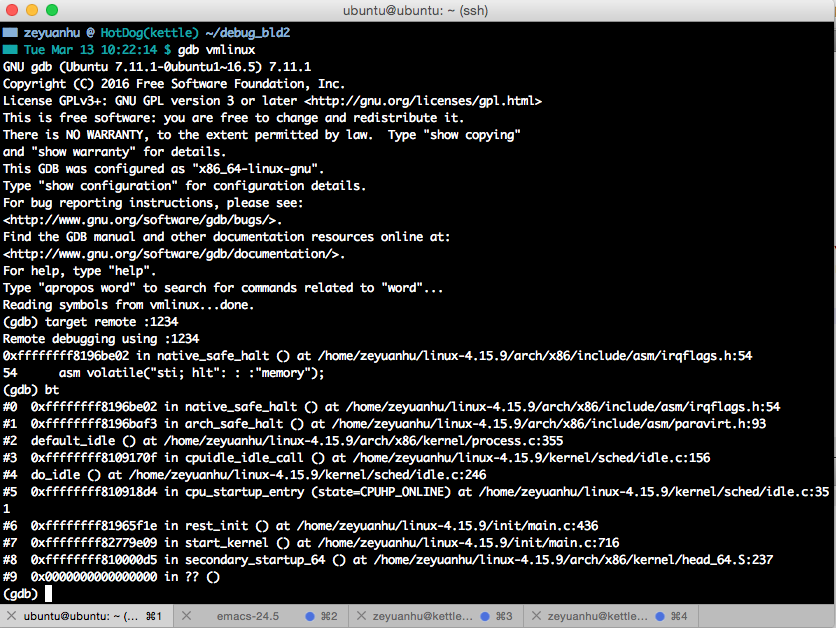
\includegraphics[scale=0.4]{gdb.png} 
\caption{Fire up GDB and be ready to debug kernel}
\label{gdb}
\end{figure}

Next, we create a program \texttt{testprog.c} on the guest system like the following
\footnote{We modify the program by appending extra line \lstinline|while (1) \{\}|. Doing so make sure that the 
breakpoint will be hit evetually when the program is being executed (since the program is non-terminal). Since the program is fairly short
and the execution is very quick. If we do not add this line, sometimes the program will finish execution without the breakpoint getting hit and
that hurts reproducibility}:

\begin{lstlisting}[style=CStyle]
#include<unistd.h>
#include<fcntl.h>
int main()
{
    int fd = open("/dev/urandom", O_RDONLY);
    char data[4096];
    read(fd, &data, 4096);
    close(fd);
    fd = open("/dev/null", O_WRONLY);
    write(fd, &data, 4096);
    close(fd);
    while (1) {}
}
\end{lstlisting}

Compile it with gcc: \lstinline|gcc -o testprog -g testprog.c|. Now, we want to trace into the kernel
when the process contains \texttt{testprog} is running
\footnote{We first run \lstinline|target remote :1234| and then we setup the breakpoint. Afterward, we issue \lstinline|continue|
in the GDB so that we can run \texttt{testprog} on the guest system.}. To do so, we set a conditional breakpoint in 
\texttt{spin\_lock} in kernel code that will only stop execution if the above process is running.
\texttt{spin\_lock} is an inline Macro and the actual symbol name is \lstinline|__raw_spin_lock|, which is
defined in \lstinline|include/linux/spinlock_api_smp.h|. To ensure the breakpoint only be triggered 
during the execution of \texttt{testprog}, we have to add a condition to the breakpoint.
We use the helper script provided by kernel to figure out the PID of \texttt{testprog}.
We achieve so via \lstinline|$lx_current()|, which reads \lstinline|task_struct| of current task in GDB
and \lstinline|task_struct| contains all the information we need to identify the current proces.
Specifically, \lstinline|$lx_current().pid| gives the PID of the current running process and 
\lstinline|$lx_current().comm| gives the command line content, which we will use it to identify the process.

% % Shows how we find the actual symbol of spin_lock
%\begin{lstlisting}
%
%// /include/linux/spinlock.h
%static __always_inline void spin_lock(spinlock_t *lock)
%{
%	raw_spin_lock(&lock->rlock);
%}
%
%// /include/linux/spinlock.h
%#define raw_spin_lock(lock)	_raw_spin_lock(lock)
%
%// /kernel/locking/spinlock.c
%void __lockfunc _raw_spin_lock(raw_spinlock_t *lock)
%{
%	__raw_spin_lock(lock);
%}
%
%// include/linux/spinlock_api_smp.h
%static inline void __raw_spin_lock(raw_spinlock_t *lock)
%{
%	preempt_disable();
%	spin_acquire(&lock->dep_map, 0, 0, _RET_IP_);
%	LOCK_CONTENDED(lock, do_raw_spin_trylock, do_raw_spin_lock);
%}
%\end{lstlisting}


The command we run is following 

\begin{lstlisting}
b __raw_spin_lock if $_streq($lx_current().comm, "testprog")
\end{lstlisting}

Figure \ref{breakpoint} shows the result of \texttt{testprog} hits the breakpoint for the first time. From the figure we can see that 
\lstinline|$lx current().pid| gives 2442 and \lstinline|$lx current().comm| gives \lstinline|"testprog\000\000\000\000\000\000\000"|, which confirm
that we are in \texttt{testprog} process when we hit \lstinline|spin_lock| breakpoint. Then, we use \lstinline|bt| to examine the call stack.

\begin{figure}
\centering
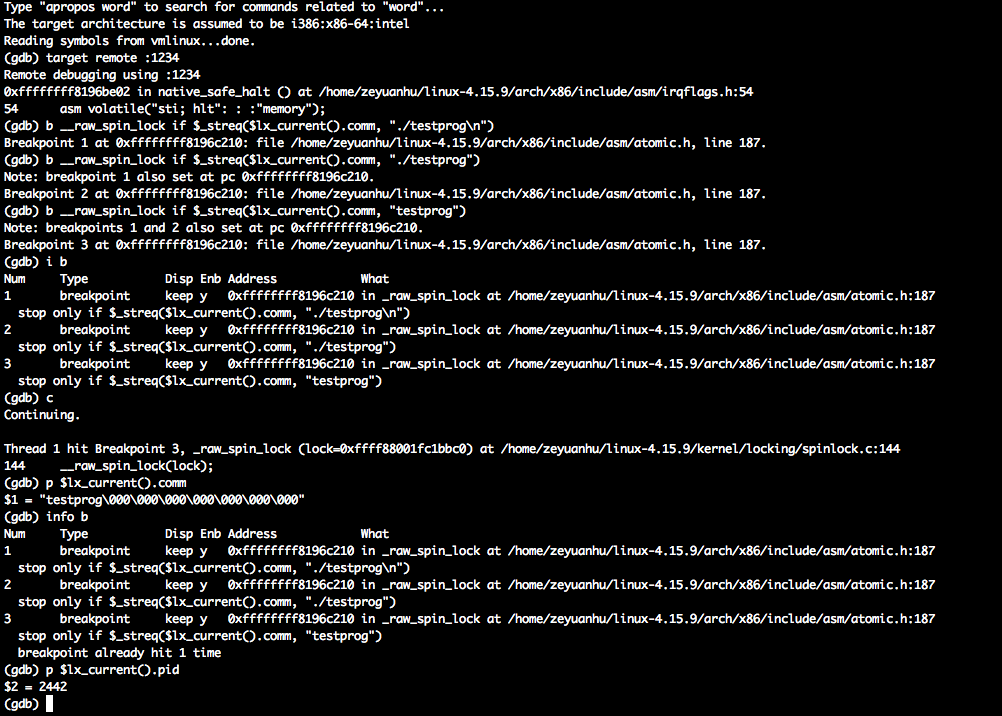
\includegraphics[scale=0.5]{breakpoint.png} 
\caption{The first time that \texttt{testprog} hits breakpoint }
\label{breakpoint}
\end{figure}

In the first time the breakpoint is triggered, the stack looks like:

\begin{lstlisting}
#0  _raw_spin_lock (lock=0xffff88001fc1bbc0) at /home/zeyuanhu/linux-4.15.9/kernel/locking/spinlock.c:144
#1  0xffffffff810bd8d0 in hrtimer_interrupt (dev=<optimized out>) at /home/zeyuanhu/linux-4.15.9/kernel/time/hrtimer.c:1303
...
\end{lstlisting}

From the tace, we see the kernel is running handler for the timer interrupt.If we take a look at function \texttt{hrtimer\_interrupt} in 
\texttt{kernel/time/hrtimer.c}, we know the \texttt{hrtimer\_bases}, a per-CPU variable \cite{cpu}, acquired a lock
\footnote{In GDB, the helper script also provides a function \lstinline|$lx_per_cpu| to obtain per-CPU variables (actually 
\lstinline|$lx_current()| is a shorthand to \lstinline|$lx_per_cpu("current task")|)}.

We continue the kernel tracing and the stack looks like below when we hit the breakpoint for the second time:

\begin{lstlisting}
#0  _raw_spin_lock (lock=0xffffffff82206a04 <jiffies_lock+4>) at /home/zeyuanhu/linux-4.15.9/kernel/locking/spinlock.c:144
...
#4  0xffffffff810cb57f in tick_sched_timer (timer=0xffff88001fc1bfe0) at /home/zeyuanhu/linux-4.15.9/kernel/time/tick-sched.c:1187
...
#9  smp_apic_timer_interrupt (regs=<optimized out>) at /home/zeyuanhu/linux-4.15.9/arch/x86/kernel/apic/apic.c:1050
\end{lstlisting}

It is still inside the handler for timer interrupt, and \lstinline|jiffies_lock| is acquired, which is a global variable. 
Function \lstinline|tick_do_update_jiffies64| updates current jiffies.

The breakpoint is hit in a different context happens inside function \texttt{update\_process\_times}, still during handler for timer interrupt:

\begin{lstlisting}
(gdb) bt
#0  _raw_spin_lock (lock=0xffff88001fc207c0) at /home/zeyuanhu/linux-4.15.9/kernel/locking/spinlock.c:144
...
#3  0xffffffff810bc9ab in update_process_times (user_tick=0) at /home/zeyuanhu/linux-4.15.9/kernel/time/timer.c:1633
...
#8  0xffffffff810bd90d in hrtimer_interrupt (dev=<optimized out>) at /home/zeyuanhu/linux-4.15.9/kernel/time/hrtimer.c:1316
\end{lstlisting}

Here the lock for per-CPU variable \texttt{runqueues} is acquired.

Continuing trace will let us see something out of timer interrupt. One example is breakpoint hit during the page fault:

\begin{lstlisting}
0  _raw_spin_lock (lock=0xffff88001cc1ec6c) at /home/zeyuanhu/linux-4.15.9/kernel/locking/spinlock.c:144
...
#3  0xffffffff81167316 in pud_alloc (address=<optimized out>, p4d=<optimized out>, mm=<optimized out>) at /home/zeyuanhu/linux-4.15.9/include/linux/mm.h:1733
#4  __handle_mm_fault (vma=<optimized out>, address=6295640, flags=<optimized out>) at /home/zeyuanhu/linux-4.15.9/mm/memory.c:4008
#5  0xffffffff811678ad in handle_mm_fault (vma=<optimized out>, address=<optimized out>, flags=<optimized out>) at /home/zeyuanhu/linux-4.15.9/mm/memory.c:4104
#6  0xffffffff8104bede in __do_page_fault (regs=0xffffc90000317ce8, error_code=2, address=6295640) at /home/zeyuanhu/linux-4.15.9/arch/x86/mm/fault.c:1426
#7  0xffffffff81a0168b in async_page_fault () at /home/zeyuanhu/linux-4.15.9/arch/x86/entry/entry_64.S:1118
\end{lstlisting}

Another one is the scheduler wakes up process and queues the process:

\begin{lstlisting}
...
#2  ttwu_queue (wake_flags=<optimized out>, cpu=<optimized out>, p=<optimized out>) at /home/zeyuanhu/linux-4.15.9/kernel/sched/core.c:1863
#3  try_to_wake_up (p=0xffff88001cf9a4c0, state=<optimized out>, wake_flags=0) at /home/zeyuanhu/linux-4.15.9/kernel/sched/core.c:2078
#4  0xffffffff8107cebc in wake_up_process (p=<optimized out>) at /home/zeyuanhu/linux-4.15.9/kernel/sched/core.c:2151
#5  0xffffffff8106d0e3 in wake_up_worker (pool=<optimized out>) at /home/zeyuanhu/linux-4.15.9/kernel/workqueue.c:840
#6  insert_work (pwq=<optimized out>, work=<optimized out>, head=<optimized out>, extra_flags=<optimized out>) at /home/zeyuanhu/linux-4.15.9/kernel/workqueue.c:1313
#7  0xffffffff8106d212 in __queue_work (cpu=<optimized out>, wq=0x0 <irq_stack_union>, work=0xffff88001fc00000) at /home/zeyuanhu/linux-4.15.9/kernel/workqueue.c:1463
#8  0xffffffff810bad36 in call_timer_fn (timer=0xffff88001fc207c0, fn=0x0 <irq_stack_union>) at /home/zeyuanhu/linux-4.15.9/kernel/time/timer.c:1318
#9  0xffffffff810bb209 in expire_timers (head=<optimized out>, base=<optimized out>) at /home/zeyuanhu/linux-4.15.9/kernel/time/timer.c:1351
#10 __run_timers (base=<optimized out>) at /home/zeyuanhu/linux-4.15.9/kernel/time/timer.c:1658
...
\end{lstlisting}

\section{Differences between \lstinline|/dev/random| and \lstinline|/dev/urandom|}

Both \lstinline|/dev/random| and \lstinline|/dev/urandom| are interfaces to the kernel's random number generator \cite{man}
and both of them are fed by the same cryptographically secure pseudorandom number generator \cite{urandom}. However, they are
different on how they handle their repective entropy pool when the pool is empty.
\lstinline|/dev/random| will block the reads if its entropy pool is empty and the reads
will be blocked until additional environmental noise is gathered. However, \lstinline|/dev/urandom| will not block waiting for
more entropy and as a result, the returned values may have theoretical vulunerability. There is an argument on when to use which
and some suggests that use \lstinline|/dev/urandom| is strictly better as the thoeretical vulunerability may not lead to 
computational vulunerability \cite{urandom} and thus should be used all the time. But, \texttt{man} page seems to suggest that
it is a case-by-case situation \cite{man}.

\end{spacing}

\bibliographystyle{ieeetr}
\bibliography{report}


\end{document}

